\documentclass{article}

\usepackage{algpseudocode}
\usepackage{booktabs}
\usepackage{caption}
\usepackage{enumitem}
\usepackage{fontspec}
\usepackage{graphicx}
\usepackage{mathtools}
\usepackage{microtype}
\usepackage{sectsty}
\usepackage[table,xcdraw]{xcolor}

\allsectionsfont{\sffamily}
\captionsetup{font=small,labelfont={bf,sf},margin=1.5em}

\title{Balanced Binary Search Trees}
\author{Florian Kretlow}

\begin{document}

\section{Red-Black-Tree}

\subsection{Introduction and general properties}
A red-black-tree is a self-balancing binary search tree. In addition to the invariants
of the latter, the former garantees that the tree remains roughly balanced even when it
receives input sequences that constitute pathological cases for normal binary search
trees (sorted input).

Every node in a red-black-tree is assigned one of two colors (traditionally red and
black). The following invariants hold after each insertion into, or deletion from a
red-black-tree.

\begin{enumerate}[label=(\arabic*)]
\item The root node of the tree is black. Every other node is either red or black.
\item If a node is red, it doesn't have a red child.
\item All paths from the root to a leaf go through the same number of black nodes.
\end{enumerate}

If \(b\) is the number of black nodes on every path from the root to a leaf, then the
shortest possible path from the root to a leaf (which contains no red nodes) has a
length of \(b\), and the longest possible path (where black and red nodes alternate) has
a length of \(2b\).  Thus the invariants ensure that the lengths of any two paths from
the root to a leaf (i.e. the depths of any two leaf nodes) differ by at most a factor of
2.

\[
\forall \text{ leaf nodes } l_{i}, l_{j} \in T : \text{depth}(l_i) \leq 2 \cdot
\text{depth}(l_j)
\]

The balance is weaker than in an AVL tree (where the difference between the heights of
the left and right sub-trees of any sub-tree is at most 1). Consequently, operations on
a red-black-tree require fewer tree rotations, so they’re faster. Both red-black-trees
and AVL trees get, insert, and delete elements in logarithmic time (\(O(\log(n))\)).

\subsection{Groups of Nodes}
Let a \emph{group} of nodes in a red-black-tree denote \emph{any black node together
with all its direct red child nodes.} Every node in a red-black-tree belongs to exactly
one group: Every black node is the ‘head’ of its own group. Every red node belongs
to the group of its black parent. Using the fact that every group contains exactly one
black node, we can rephrase invariant 3 as follows:

\begin{enumerate}[label=(\arabic*)]
\setcounter{enumi}{2}
\item All paths from the root to a leaf go through the same number of groups.
\end{enumerate}

The \emph{weight} of a group \(g\) is the number of nodes it contains, obviously \(1
\leq \text{weight}(g) \leq 3\). If \(\text{weight}(g) = 1\), \(g\) is said to be
\emph{empty:} it doesn't contain any red child nodes.  If \(\text{weight}(g) = 3\),
\(g\) is said to be \emph{full:} it contains two red child nodes and it's not possible
to add another node to the group.  If \(\text{weight}(g) = 2\), it's possible to rotate
\(g\) in such a way that the former red child becomes the black root of the group, and
the former black root becomes a red child on the opposite site; this rotation does not
affect any other group than \(g\).

\begin{figure}
\begin{centering}
    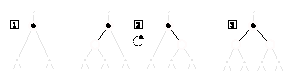
\includegraphics[scale=2]{img/groups.pdf}
    \caption{Possible groups in a red-black-tree. The direct ancestor of the head of a
    group can be both red and black. Every direct descendant below a group is black.}
\end{centering}
\end{figure}

\subsection{Insertion}
Insertion into a normal binary search tree is straightforward. You start at the root,
and then you always go left if the new value is less than the current value, or you go
right if it is greater. When you've nowhere left to go (i.e. you'd need to go left but
there's no left child, or the other way around) you simply add the value at that
position.

In order to preserve the invariants, inserting a node into a red-black-tree must not add
a new group to the tree (except at the very root where the addition affects all paths
equally).  Therefore insertion is not possible if the direct parent of the to-be-added
node is part of a full group. The solution is to reduce the weight of that group: If \(
\text{weight}(g) \leq 2\), it is possible to add a node to \(g\).

\begin{small}
\begin{verbatim}
procedure decrease-weight(n):
    p := parent of n
    pp := grandparent of n
    l, r := children of n

    // assume that n is black and l, r are red

    case 1: n is the root of the tree
        recolor:
            l, r: black

    case 2: p is black
        recolor:
            n: red
            l, r: black

    case 3: p is red
        case 3.1: pp has 1 red child (p)
            case 3.1a: pp->p->n is right-right or left-left
                right-right: rotate-left(pp)
                left-left: rotate-right(pp)
                recolor:
                    pp: red
                    p: black
                    n: red
                    l, r: black
            case 3.1b: pp->p->n is right-left or left-right
                right-left:
                    rotate-right(p)
                    rotate-left(pp)
                left-right:
                    rotate-left(p)
                    rotate-right(pp)
                recolor:
                    pp: red
                    l, r: black

        case 3.2: pp has 2 red children
            decrease-weight(pp)
            decrease-weight(n) // try again

procedure insert(n, v):
    p := parent of n

    if v == n.value:
        return
    else if v < n.value and n has a left child:
        insert(n.left, v)
        return
    else if v > n.value and n has a right child:
        insert(n.right, v)
        return

    case 1: n is black
        if v < n.value:
            n.left = new node(v, red)
            n.left.parent = n
        else:
            n.right = new node(v, red)
            n.right.parent = n

    case 2: n is red
        case 2.1: weight(p) = 2
            decrease-weight(p)
            // now n can be anywhere, go again:
            insert(n, v)

        case 2.2: weight(p) = 1
            case 2.2.1: v < n.value and n = p.left
                rotate-right(p)
                n.left = new node(v, red)
            case 2.2.2: v > n.value and n = p.right
                rotate-left(p)
                n.right = new node(v, red)
            case 2.2.3: v < n.value and n = p.right
                p.left = new node(v, red)
                swap(p, p.left)
            case 2.2.4: v > n.value and n = p.left
                p.right = new node(v, red)
                swap(p, p.right)
\end{verbatim}
\end{small}

\subsection{Deletion}
Deletion is only possible if the group we delete from is not empty. Likewise, deleting a node from the tree must not remove a group entirely
(again, except at the root).

\begin{small}
\begin{verbatim}
procedure increase-weight(n):
    p := parent of n
    s := sibling of n

    // case 1: ancestor group is not empty
    if p is red or weight(p) >= 2:
        if p is black:
            if n == p.right:
                rotate-right(p); s = p.left
            else:
                rotate-left(p); s = p.right

        // case 1.1: s is empty
        if weight(s) == 1:
            recolor:
                p: black
                n, s: red

        // case 1.2: s is not empty
        else:
            // make sure s has an outer child
            if s == p.left and s.left is black:
                rotate-left(s); s = p.left
            else if s == p.right and s.right is black:
                rotate-right(s); s = p.right

            if n == p.right:
                rotate-right(p)
            else:
                rotate-left(p)

            recolor:
                p: black
                n, s: red
                outer child of s: black

    // case 2: ancestor group is empty
    else:
        // case 2.1: s is empty
        if weight(s) == 1:
            if p is root:
                recolor:
                    n, s: red
            else:
                increase-weight(p)
                increase-weight(n)

        // case 2.2: s is not empty
        else:
            // make sure s has an outer child
            if s == p.left and s.left is black:
                rotate-left(s); s = p.left
            else if s == p.right and s.right is black:
                rotate-right(s); s = p.right

            if n == p.right:
                rotate-right(p)
            else:
                rotate-left(p)

            recolor:
                n: red
                outer child of s: black


procedure delete(n, v):
    while v != n.value:
        if v < n.value:
            n = n.left
        else if v > n.value:
            n = n.right
        if n == nil: return // not found

    if n is not in a leaf position:
        successor := n.right
        while successor has a left child:
            successor = successor.left
        swap(n, successor)
        // now n is where successor was, in a leaf position

    if n is black and not the root and weight(n) == 1:
        increase-weight(n)

    if n is black:
        if n has a left child:
            rotate-right(n)
        else:
            rotate-left(n)

    remove n from the tree

\end{verbatim}
\end{small}

\end{document}
